\documentclass{beamer}
\usepackage{graphicx}
\usepackage{verbatim}
\usepackage{amsmath}
\usepackage{amsfonts}
\usepackage{setspace}
% \usepackage{beamerthemesplit} // Activate for custom appearance

\title{Inference in Normal Regression Model}
\author{Dr. Frank Wood}

\date{}

\DeclareMathOperator*{\Ave}{\mathbb{E}}
\DeclareMathOperator*{\Var}{Var}

\begin{document}

\frame{\titlepage}



\frame[t] {
 \frametitle{Remember}
\begin{itemize}
\item We know that the point estimator of $b_1$ is 
$$b_1=  \frac{\sum(X_i-\bar X)(Y_i - \bar Y)}{\sum(X_i - \bar X)^2}$$
\item Last class we derived the sampling distribution of $b_1$, it being $N(\beta_1,Var(b_1))$(when $\sigma^2$ known) with
$$\Var(b_1) = \sigma^2\{b_1\} = \frac{\sigma^2}{\sum(X_i - \bar X)^2}$$
\item And we suggested that an estimate of $\Var(b_1)$ could be arrived at by substituting the MSE for $\sigma^2$ when $\sigma^2$ is unknown.
$$s^2\{b_1\} = \frac{MSE}{\sum(X_i - \bar X)^2} = \frac{\frac{SSE}{n-2}}{\sum(X_i - \bar X)^2}$$
\end{itemize}
}

\frame[t] {
 \frametitle{Sampling Distribution of $(b_1 - \beta_1)/s\{b_1\}$}
\begin{itemize}
\item Since $b_1$ is normally distribute, $(b_1 - \beta_1)/\sigma\{b_1\}$ is a standard normal variable $N(0,1)$
\item We don't know $\Var(b_1)$ so it must be estimated from data.  We have already denoted it's estimate
$s^2\{b_1\}$
\item Using this estimate we it can be shown that
$$\frac{b_1-\beta_1}{s\{b_1\}} \sim t(n-2)$$
where
$$s\{b_1\} = \sqrt{ s^2\{b_1\}}$$
\end{itemize}
It is from this fact that our confidence intervals and tests will derive.
}

\frame[t] {
 \frametitle{Where does this come from?}
\begin{itemize}
\item We need to rely upon (but will not derive) the following theorem\\
\bigskip
For the normal error regression model
$$\frac{SSE}{\sigma^2} = \frac{\sum (Y_i - \hat Y_i)^2}{\sigma^2} \sim \chi^2(n-2)$$
and is independent of $b_0$ and $b_1$.\\
\bigskip
\item Here there are two linear constraints
\begin{eqnarray*}
b_1 &=&  \frac{\sum(X_i-\bar X)(Y_i - \bar Y)}{\sum(X_i - \bar X)^2} = \sum_i k_i Y_i,\;\;\; k_i = \frac{X_i - \bar X}{\sum_i (X_i - \bar X)^2}\\
b_0 &=& \bar Y - b_1 \bar X
\end{eqnarray*}

 imposed by the regression
parameter estimation that each reduce the number of degrees of
freedom by one (total two).
\end{itemize}
}

\frame[t] {
 \frametitle{Reminder: normal (non-regression) estimation}
\begin{itemize}
\item Intuitively the regression result from the previous slide follows the standard result for the sum of squared standard normal random variables.  First, with $\sigma$ and $\mu$ known
$$\sum_{i=1}^n Z_i^2 = \sum_{i=1}^n \left( \frac{Y_i-\mu}{\sigma} \right)^2 \sim \chi^2(n)$$
and then with $\mu$ unknown
\begin{eqnarray*}
S^2 &=& \frac{1}{n-1} \sum_{i=1}^n (Y_i-\bar Y)^2 \\
\frac{(n-1)S^2}{\sigma^2} &=& \sum_{i=1}^n \left( \frac{Y_i-\bar Y}{\sigma} \right)^2 \sim \chi^2(n-1)
\end{eqnarray*}
and $\bar Y$ and $S^2$ are independent. \footnote{Wackerly, pg. 335}
\end{itemize}
}

\frame[t] {
 \frametitle{Reminder: normal (non-regression) estimation cont.}
\begin{itemize}
\item With both  $\mu$ and $\sigma$ unknown then
$$ \sqrt{n}\left(\frac{\bar Y - \mu}{S}\right) \sim t(n-1) $$
\end{itemize}

because
$$ T = \frac{Z}{\sqrt{W/\nu}} = \frac{ \sqrt{n}(\bar Y - \mu)/\sigma}{\sqrt{[(n-1)S^2/\sigma^2]/(n-1)}} = \sqrt{n}\left(\frac{\bar Y - \mu}{S}\right) $$
\bigskip
Here the numerator follows from 
$$ Z = \frac{\bar Y - \mu_{\bar Y}}{\sigma_{\bar Y}} = \frac{\bar Y - \mu}{\sqrt{\frac{\sigma^2}{n}}}$$

}

\frame[t] {
 \frametitle{Another useful fact : Student-t distribution}
Let $Z$ and $\chi^2(\nu)$ be independent random variables (standard
normal and $\chi^2$ respectively).  We then define a t random
variable as follows:
$$t(\nu) = \frac{Z}{\sqrt{\frac{\chi^2(\nu)}{\nu}}}$$
This version of the t distribution has one parameter, the degrees of
freedom $\nu$

}

\frame[t] {
 \frametitle{Distribution of the studentized statistic}
To derive the distribution of the statistic $\frac{b_1 - \beta_1}{s\{b_1\}} $ first we do the
following rewrite
$$\frac{b_1 - \beta_1}{s\{b_1\}} = \frac{\frac{b_1 - \beta_1}{{ \sigma\{b_1\}}}}{\frac{s\{b_1\}}{ \sigma\{b_1\} }}$$
where
$$\frac{s\{b_1\}}{ \sigma\{b_1\} }= \sqrt{\frac{s^2\{b_1\}}{ \sigma^2\{b_1\} }}$$}

\frame[t] {
 \frametitle{Studentized statistic cont.}
And note the following
$$\frac{s^2\{b_1\}}{ \sigma^2\{b_1\} }= \frac{\frac{MSE}{\sum(X_i-\bar X)^2}}{\frac{\sigma^2}{\sum(X_i-\bar X)^2}} = \frac{MSE}{\sigma^2} = \frac{SSE}{\sigma^2(n-2)}$$
where we know (by the given theorem) the distribution of the last
term is $\chi^2$ and indep. of $b_1$ and $b_0$
$$\frac{SSE}{\sigma^2(n-2)} \sim \frac{\chi^2(n-2)}{n-2}$$}

\frame[t] {
 \frametitle{Studentized statistic final}
But by the given definition of the t distribution we have our result
$$\frac{b_1-\beta_1}{s\{b_1\}} \sim t(n-2)$$
because putting everything together we can see that $$\frac{b_1 -
\beta_1}{s\{b_1\}} \sim
\frac{z}{\sqrt{\frac{\chi^2(n-2)}{n-2}}}$$ }

\frame[t] {
 \frametitle{Confidence Intervals and Hypothesis Tests}
Now that we know the sampling distribution of $b_1$ (t with n-2
degrees of freedom) we can construct confidence intervals and
hypothesis tests easily }


\frame[t] {%%%change pic%%%
 \frametitle{Confidence Interval for $\beta_1$}
Since the ``studentized'' statistic follows a t distribution we can
make the following probability statement
$$P(t(\alpha/2; n-2)  \leq \frac{b_1-\beta_1}{s\{b_1\}}  \leq t(1-\alpha/2; n-2) ) = 1- \alpha$$
\begin{figure}
  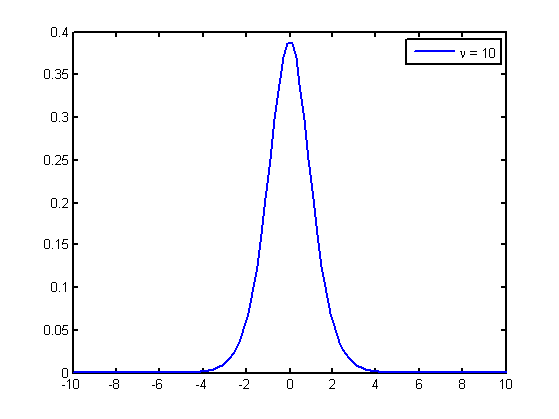
\includegraphics[height=20mm]{1.png}
  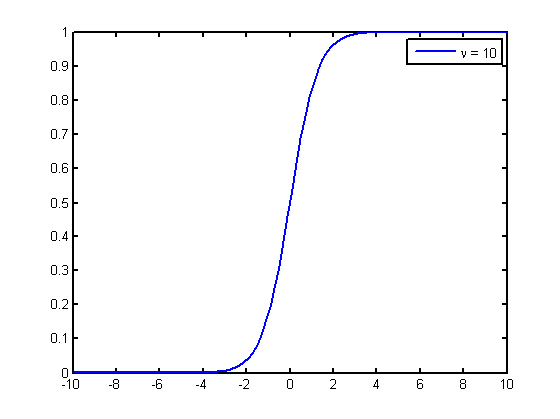
\includegraphics[height=20mm]{2.png}
  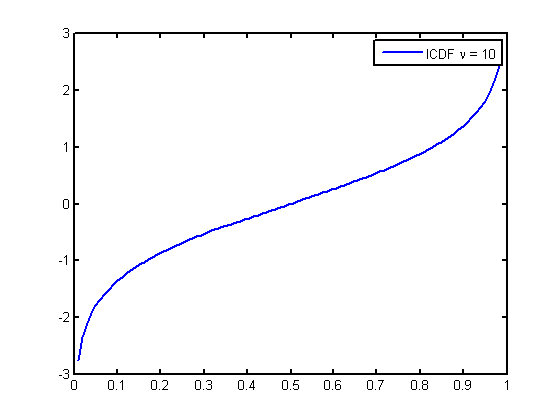
\includegraphics[height=20mm]{3.png}
\end{figure}
}

\frame[t] {
 \frametitle{Remember}
\begin{itemize}
\item Density: $f(y) = \frac{dF(y)}{dy}$
\item Distribution (CDF): $F(y) = P(Y \leq y) = \int_{-\infty}^yf(t)dt$
\item Inverse CDF: $F^{-1}(p) = y \;\; \mbox{s.t.} \;\; \int_{-\infty}^yf(t)dt = p$
\end{itemize}
}

\frame[t] {
 \frametitle{Interval arriving from picking $\alpha$}
\begin{itemize}
\item Note that by symmetry $$t(\alpha/2; n-2) = -t(1-\alpha/2; n-2)$$
\item Rearranging terms and using this fact we have
$P(b_1 - t(1-\alpha/2; n-2 )s\{b_1\} \leq \beta_1  \leq b_1 +
t(1-\alpha/2; n-2 ) s\{b_1\}) = 1- \alpha$
\item And now we can use a table to look up and produce confidence intervals
\end{itemize}
}

\frame[t] {
 \frametitle{Using tables for Computing Intervals }
\begin{itemize}
\item The tables in the book (table B.2 in the appendix) for $t(1-\alpha/2;\nu)$ where
$P\{t(\nu)\leq t(1-\alpha/2;\nu)\} = A$
\item Provides the inverse CDF of the t-distribution
\item This can be arrived at computationally as well\\
Matlab: $tinv(1-\alpha/2, \nu)$
\end{itemize}
}

\frame[t] {
 \frametitle{$1-\alpha$ confidence limits for $\beta_1$}
\begin{itemize}
\item The $1-\alpha$ confidence limits for $\beta_1$ are
$$b_1 \pm  t(1-\alpha/2; n-2 )s\{b_1\}$$
\item Note that this quantity can be used to calculate confidence intervals given n and $\alpha$.
\begin{itemize}
\item Fixing $\alpha$ can guide the choice of sample size if a particular confidence interval is desired
\item Give a sample size, vice versa.
\end{itemize}
\item Also useful for hypothesis testing
\end{itemize}
}

\frame[t] {
 \frametitle{Tests Concerning $\beta_1$}
\begin{itemize}
\item Example 1
\begin{itemize}
\item Two-sided test
\begin{itemize}
\item $H_0 : \beta_1 = 0$
\item $H_a : \beta_1 \neq 0$
\item Test statistic
$$t^* = \frac{b_1-0}{s\{b_1\} }$$
\end{itemize}
\end{itemize}
\end{itemize}
}

\frame[t] {
 \frametitle{Tests Concerning $\beta_1$}
\begin{itemize}
\item We have an estimate of the sampling distribution of $b_1$ from the data.
\item If the null hypothesis holds then the $b_1$ estimate coming from the data
should be within the $95\%$ confidence interval of the sampling
distribution centered at 0 (in this case)
$$t^* = \frac{b_1-0}{s\{b_1\} }$$
\end{itemize}
}

\frame[t] {
 \frametitle{Decision rules}
\begin{eqnarray*}
\mathrm{if }\,  |t^*| &\leq& t(1-\alpha/2;n-2)\mathrm{, conclude } \, H_0\\
\mathrm{if }\,  |t^*| &>& t(1-\alpha/2;n-2)\mathrm{, conclude }\,
H_\alpha
\end{eqnarray*}
Absolute values make the test two-sided }

\frame[t] {%%%change pic%%%
 \frametitle{Intuition}
\begin{figure}
  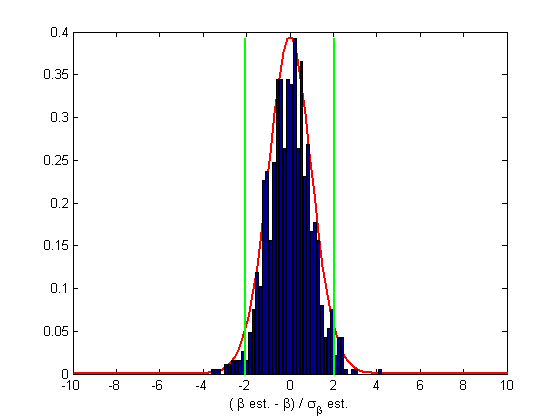
\includegraphics[height=60mm]{intuition.png}
\end{figure}
p-value is value of $\alpha$ that moves the green line to the blue
line }

\frame[t] {
 \frametitle{Calculating the p-value}
\begin{itemize}
\item The p-value, or attained significance level, is the smallest level of significance $\alpha$
for which the observed data indicate that the null hypothesis should be rejected.
\item This can be looked up using the CDF of the test statistic.
\item In Matlab\\
Two-sided p-value\\
$2*(1-tcdf(|t^*|,\nu))$

\end{itemize}
}

\frame[t] {
 \frametitle{Inferences Concerning $\beta_0$}
\begin{itemize}
\item Largely, inference procedures regarding $\beta_0$ can be performed in the same way as those
for $\beta_1$
\item Remember the point estimator $b_0$ for $\beta_0$
$$b_0 = \bar Y - b_1 \bar X$$
\end{itemize}
}

\frame[t] {
 \frametitle{Sampling distribution of $b_0$}
\begin{itemize}
\item The sampling distribution of $b_0$ refers to the different values of $b_0$
that would be obtained with repeated sampling when the levels of the
predictor variable X are held constant from sample to sample.
\item For the normal regression model the sampling distribution of $b_0$ is normal

\end{itemize}
}

\frame[t] {
 \frametitle{Sampling distribution of $b_0$}
\begin{itemize}
\item When error variance is known
$$\Ave(b_0) = \beta_0$$
$$\sigma^2\{b_0\} = \sigma^2 (\frac{1}{n} + \frac{\bar X^2}{\sum(X_i - \bar X)^2})$$
\item When error variance is unknown
$$s^2\{b_0\}= MSE (\frac{1}{n} + \frac{\bar X^2}{\sum(X_i - \bar
X)^2})$$
\end{itemize}
}

\frame[t] {
 \frametitle{Confidence interval for $\beta_0$}
The $1-\alpha$ confidence limits for $\beta_0$ are obtained in the
same manner as those for $\beta_1$
$$b_0 \pm  t(1-\alpha/2; n-2 )s\{b_0\}$$
}

\frame[t] {
 \frametitle{Considerations on Inferences on $\beta_0$ and $\beta_1$}
\begin{itemize}
\item Effects of departures from normality\\
The estimators of $\beta_0$ and $\beta_1$ have the property of
asymptotic normality - their distributions approach normality as the
sample size increases (under general conditions)
\item Spacing of the X levels
The variances of $b_0$ and $b_1$ (for a given n and $\sigma^2$)
depend strongly on the spacing of X

\end{itemize}
}

\frame[t] {
 \frametitle{Sampling distribution of point estimator of mean response}
\begin{itemize}
\item Let $X_h$ be the level of X for which we would like an estimate of the mean
response\\
Needs to be one of the observed X's
\item The mean response when $X=X_h$ is denoted by $\Ave(Y_h)$
\item The point estimator of $\Ave(Y_h)$ is
$$\hat Y_h = b_0 + b_1 X_h$$
We are interested in the sampling distribution of this quantity
\end{itemize}
}

\frame[t] {
 \frametitle{Sampling Distribution of $\hat Y_h$}
\begin{itemize}
\item We have
$$\hat Y_h = b_0 + b_1 X_h$$
\item Since this quantity is itself a linear combination of the $Y_i's$ it's sampling distribution is itself normal.
\item The mean of the sampling distribution is $$E\{\hat Y_h\} = E\{b_0\} + E\{b_1\} X_h = \beta_0 + \beta_1X_h$$
Biased or unbiased?
\end{itemize}
}

\frame[t] {
 \frametitle{Sampling Distribution of $\hat Y_h$}
\begin{itemize}
\item To derive the sampling distribution variance of the mean response we first show that
$b_1$ and $(1/n)\sum Y_i$ are uncorrelated and, hence, for the
normal error regression model independent
\item We start with the definitions
$$\bar Y = \sum (\frac{1}{n}) Y_i$$
\begin{eqnarray*}
b_1 &=& \sum k_i Y_i, \, k_i = \frac{(X_i - \bar X)}{\sum(X_i-\bar
X)^2}
\end{eqnarray*}

\end{itemize}
}

\frame[t] {
 \frametitle{Sampling Distribution of $\hat Y_h$}
\begin{itemize}
\item We want to show that mean response and the estimate $b_1$ are uncorrelated
$$Cov(\bar Y, b_1) = \sigma^2\{\bar Y, b_1\} = 0$$
\item To do this we need the following result (A.32)
$$\sigma^2\{\sum_{i=1}^n a_i Y_i, \sum_{i=1}^n c_i Y_i\} = \sum_{i=1}^n a_i c_i \sigma^2\{Y_i\}$$
when the $Y_i$ are independent
\end{itemize}
}


\frame[t] {
 \frametitle{Sampling Distribution of $\hat Y_h$}
Using this fact we have
\begin{eqnarray*}
\sigma^2\{\sum_{i=1}^n \frac{1}{n} Y_i, \sum_{i=1}^n k_i Y_i\} &=& \sum_{i=1}^n \frac{1}{n} k_i \sigma^2\{Y_i\} \\
&=&  \sum_{i=1}^n \frac{1}{n} k_i \sigma^2 \\
&=& \frac{\sigma^2 }{n}  \sum_{i=1}^n k_i \\
&=& 0
\end{eqnarray*}
So the $\bar{Y}$ and $b_1$ are uncorrelated }

\frame[t] {
 \frametitle{Sampling Distribution of $\hat Y_h$}
\begin{itemize}
\item This means that we can write down the variance
$$\sigma^2\{\hat Y_h\} = \sigma^2\{\bar Y + b_1(X_h - \bar X)\}$$
alternative and equivalent form of regression function
\item But we know that the mean of Y and $b_1$ are uncorrelated so
$$\sigma^2\{\hat Y_h\} = \sigma^2\{\bar Y\} + \sigma^2\{b_1\}(X_h - \bar X)^2$$
\end{itemize}
}

\frame[t] {
 \frametitle{Sampling Distribution of $\hat Y_h$}
\begin{itemize}
\item We know (from last lecture)
\begin{eqnarray*}
\sigma^2\{b_1\} &=&  \frac{\sigma^2}{\sum(X_i - \bar X)^2} \\
s^2\{b_1\} &=&  \frac{MSE}{\sum(X_i - \bar X)^2}
\end{eqnarray*}
\item And we can find
$$\sigma^2\{\bar Y\} = \frac{1}{n^2} \sum  \sigma^2\{Y_i\} =  \frac{n \sigma^2 }{n^2} =   \frac{ \sigma^2 }{n}$$
\end{itemize}
}

\frame[t] {
 \frametitle{Sampling Distribution of $\hat Y_h$}
\begin{itemize}
\item So, plugging in, we get
$$\sigma^2\{\hat Y_h\} = \frac{\sigma^2}{n}+ \frac{\sigma^2}{\sum(X_i - \bar X)^2}(X_h - \bar X)^2$$
\item Or
$$\sigma^2\{\hat Y_h\} = \sigma^2\left(\frac{1}{n}+ \frac{(X_h - \bar X)^2 }{\sum(X_i - \bar X)^2}\right)$$
\end{itemize}
}

\frame[t] {
 \frametitle{Sampling Distribution of $\hat Y_h$}
Since we often won't know $\sigma^2$ we can, as usual, plug in $S^2
= SSE/(n-2)$, our estimate for it to get our estimate of this
sampling distribution variance $$s^2\{\hat Y_h\} =
S^2\left(\frac{1}{n}+ \frac{(X_h - \bar X)^2 }{\sum(X_i - \bar
X)^2}\right)$$ }

\frame[t] {
 \frametitle{No surprise$\ldots$}
\begin{itemize}
\item The sampling distribution of our point estimator for the output is distributed as a t-distribution with two degrees of freedom
$$\frac{\hat Y_h - E\{Y_h\}}{s\{\hat Y_h\}} \sim t(n-2)$$
\item This means that we can construct confidence intervals in the same manner as before.
\end{itemize}
}

\frame[t] {
 \frametitle{Confidence Intervals for $\Ave(Y_h)$}
\begin{itemize}
\item The $1-\alpha$ confidence intervals for $\Ave(Y_h)$ are
$$\hat Y_h \pm t(1-\alpha/2; n-2)s\{\hat Y_h\}$$
\item From this hypothesis tests can be constructed as usual.

\end{itemize}
}

\frame[t] {
 \frametitle{Comments}
\begin{itemize}
\item The variance of the estimator for$\Ave(Y_h)$ is smallest near the mean of X.
Designing studies such that the mean of X is near $X_h$ will improve
inference precision
\item When $X_h$ is zero the variance of the estimator for $\Ave(Y_h)$ reduces to the variance of the estimator $b_0$ for
$\beta_0$
\end{itemize}
}

\frame[t] {
 \frametitle{Prediction interval for single new observation}
\begin{itemize}
\item Essentially follows the sampling distribution arguments for $\Ave(Y_h)$
\item If all regression parameters are known then the $1-\alpha$ prediction interval for a new observation $Y_h$ is
$$\Ave\{Y_h\} \pm z(1-\alpha/2)\sigma$$
\end{itemize}
}

\frame[t] {
 \frametitle{Prediction interval for single new observation}
\begin{itemize}
\item If the regression parameters are unknown the $1-\alpha$ prediction interval for a new observation $Y_h$ is given by the following theorem
$$\hat Y_h \pm t(1-\alpha/2; n-2){s\{pred\}}$$
\item This is very nearly the same as prediction for a known value of X but includes a correction for
the fact that there is additional variability arising from the fact
that the new input location was not used in the original estimates
of $b_1$, $b_0$, and $s^2$
\end{itemize}
}

\frame[t] {
 \frametitle{Prediction interval for single new observation}
The value of $s^2\{pred\}$ is given by
$${s^2\{pred\}}  = MSE\left[ 1 + \frac{1}{n} + \frac{(X_h-\bar X)^2}{\sum (X_i - \bar X)^2}\right]$$
}



\end{document}
